\begin{figure}[H]
    \centering
    \definecolor{moveblue}{RGB}{45,115,180}
    \definecolor{initialgray}{RGB}{115,120,125}
    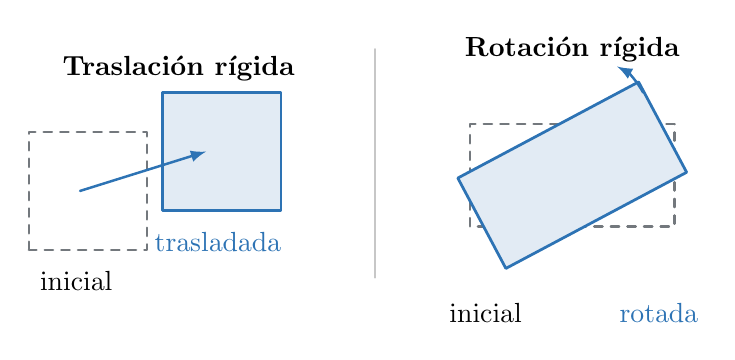
\begin{tikzpicture}[x=1cm,y=1cm,line cap=round,line join=round]
        \node[font=\bfseries] at (2.5,3.1) {Traslación rígida};
        \draw[initialgray,dashed,line width=0.9pt] (0.6,0.8) rectangle (2.1,2.3);
        \fill[moveblue!14] (2.3,1.3) rectangle (3.8,2.8);
        \draw[moveblue,line width=1pt] (2.3,1.3) rectangle (3.8,2.8);
        \draw[moveblue,-latex,line width=0.9pt] (1.25,1.55) -- (2.85,2.05);
        \node[below] at (1.2,0.65) {inicial};
        \node[below,text=moveblue] at (3.0,1.15) {trasladada};

        \draw[black!22,line width=0.7pt] (5.0,0.45) -- (5.0,3.35);

        \node[font=\bfseries] at (7.5,3.35) {Rotación rígida};
        \draw[initialgray,dashed,line width=0.9pt] (6.2,1.1) rectangle (8.8,2.4);
        \begin{scope}[shift={(7.5,1.75)},rotate=28]
            \fill[moveblue!14] (-1.3,-0.65) rectangle (1.3,0.65);
            \draw[moveblue,line width=1pt] (-1.3,-0.65) rectangle (1.3,0.65);
        \end{scope}
        \draw[moveblue,-latex,line width=0.9pt] (8.4,2.8) arc[start angle=28,end angle=62,radius=0.8];
        \node[below] at (6.4,0.25) {inicial};
        \node[below,text=moveblue] at (8.6,0.25) {rotada};
    \end{tikzpicture}
    \caption{La traslación y la rotación cambian posición u orientación, pero no deforman el cuerpo.}
\end{figure}